\documentclass{thesis}

\title{硒化镉量子点的二维光谱探测}
\author{陈稼霖} % 学生姓名
\id{45875852} % 学号
\entranceYear{2017} % 入学年份
\institute{物质科学与技术学院} % 院系名称
\major{物理学} % 二级学科专业名称
\advisor{John A. McGuire} % 指导教师:姓名
\date{二零二一~年~六~月} % 毕业日期:夏季为6月、冬季为12月

\titleEn{Two-dimensional Spectroscopy of \text{CdSe} Quantum Dots}% Title
\authorEn{Jialin Chen}% Student name
\instituteEn{School of Physical Science and Technology}% 院系名称
\majorEn{Physics}% 二级学科专业名称
\advisorEn{John A. McGuire}% Advisor
\dateEn{June / 2021}% 毕业日期:夏季为June、冬季为December

\begin{document}
\frontmatter
\maketitle
\maketitleEn
\makedeclaration
\makeabstract{% 中文摘要
    二维光谱是一种基于四波混频效应的超快激光光谱技术。它用三个激光脉冲组成的序列激励材料,得到以泵浦和探测频率为自变量的非线性光学响应谱。相较传统一维光谱,二维光谱能够揭示材料更为丰富的信息:其对角峰反映了材料的能级分布,而非对角峰则反映了能级间的耦合关系。本项目以硒化镉量子点这一具有分立能级且研究得较为透彻的材料为样品,利用二维电子光谱研究的其电子动力学机制。我们首先利用紫外可见吸收光谱获得了硒化镉量子点的能级分布的大致情况,然后通过瞬态吸收谱确定了产生单激子激发的泵浦能量范围,在确保单激子激发的前提下,我们测量了硒化镉量子点的二维光谱,分析其信号峰的分布、展宽等特征蕴含的信息。
}{% 中文关键词
    二维光谱,硒化镉量子点,四波混频
}%它以脉冲间时延经傅里叶变换得到的频率和/或脉冲光本身的频率为自变量,以材料的非线性光学响应为因变量
\makeenglishabstract{% English abstract
    Two-dimensional spectroscopy is an ultrafast laser spectroscopy technology based on four-wave mixing effect. It excites the material with sequences of three laser pulses, and obtains a non-linear optical response spectrum with pump and probe frequencies as variables. Compared with traditional one-dimensional spectroscopy, two-dimensional spectroscopy can reveal richer information of materials: its diagonal peaks reflect the energy level distribution of the materials, while non-diagonal peaks reflect the coupling relationship between the energy levels. This project takes cadmium selenide quantum dots, a material that has discrete energy levels and has been studied thoroughly, as sample, and uses two-dimensional electronic spectroscopy to study its electronic dynamics mechanism. We first obtained the general situation of the energy level distribution of the cadmium selenide quantum dots with ultraviolet-visible absorption spectrum, and then determined the pump energy range for single-exciton regime. In single exciton regime, We measured the two-dimensional spectrum of cadmium selenide quantum dots and analyzed the information contained in the signal peak distribution, broadening and other characteristics.
}{% English key words
    Two-dimensional spectroscopy, CdSe quantum dots, four-wave mxing
}
\begin{spacing}{1}
    \zihao{5}\tableofcontents
    \thispagestyle{empty}
\end{spacing}
\mainmatter
\chapter{背景介绍}
\thispagestyle{firstpagestyle}

\section{二维光谱的基本原理 --- 四波混频}
二维光谱是基于四波混频(Four-wave Mixing,简称 FWM)研究待测体系能级间相互作用的一种光谱测量手段。

四波混频效应是一种三阶非线性光学效应。该效应是指,两束或三束不同波长的光入射非线性介质,产生新的波长的信号光。以最一般的一种情况为例:系统中的粒子具有如图 ? 所示的 $V$ 型能级结构,三个能级分别为 $\lvert 1\rangle$, $\lvert 2\rangle$, $\lvert 3\rangle$。如图 \ref{Four-wave Mixing} 所示,假设标号为 $1$, $2$, $3$ 的三束电磁波分别以 $\hat{k}_1$, $\hat{k}_2$, $\hat{k}_3$ 角度入射待测系统。

\begin{figure}[h]
    \centering
    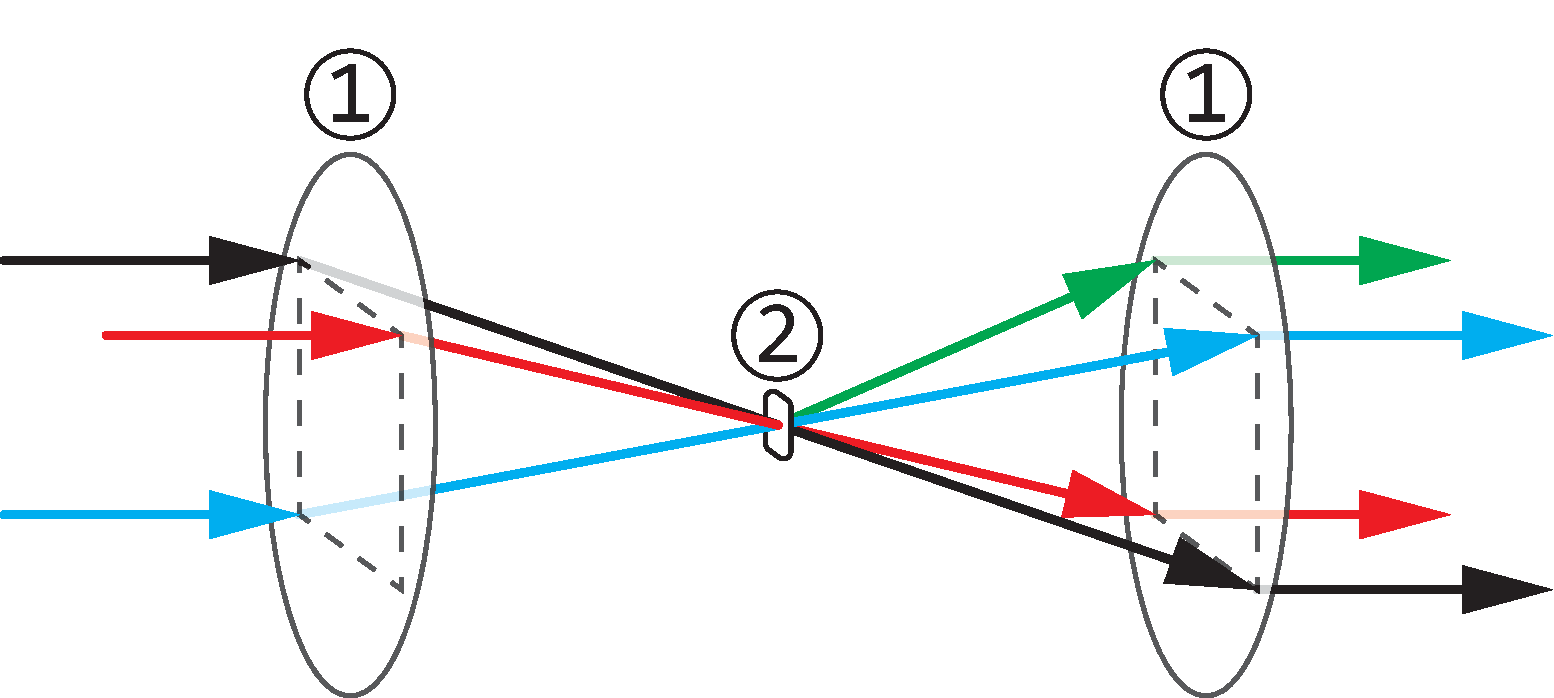
\includegraphics[width=.5\columnwidth]{Img/Four-wave Mixing.pdf}
    \caption{四波混频示意图,其中:\textcircled{\footnotesize{1}} --- 凸透镜,\textcircled{\footnotesize{2}} --- 待测体系。标号为 $1$, $2$, $3$ 的三束不同波长的光分别经一凸透镜聚焦,由 $\bm{k}_1$, $\bm{k}_2$, $\bm{k}_3$ 方向入射于待测体系,出射光中除了有以上三束光的透射以外,在 $\bm{k}_3+\bm{k}_2-\bm{k}_1$ 方向上还将产生一个新的波长的光。}
    \label{Four-wave Mixing}
\end{figure}

假设体系中的各个原子均被固定各自的位置上,因此在无外加光场入射的情况下,平衡状态下体系格粒子遵循玻尔兹曼分布(即使对于全同粒子,在定域的情况下,也可以认为是能够被相互分辨的,在本实验中,飞秒级别的超快激光脉冲通过样品的时间极短,在此时间内可以近似认为样品中的量子点处于静止状态,因此适用于这一模型),密度矩阵可以表示为
\begin{align}
    \hat{\rho}^{(0)}(t=0)=\lvert g\rangle\langle g\rvert.
\end{align}

三束光的电场分量可以分别表示为
\begin{align}
    \bm{E}_n(\bm{r},t)=[E_n(t)e^{i(\bm{k}_1\cdot\bm{r}-\omega_1t)}+\text{c.c.}]\hat{e},\quad n=1,2,3.
\end{align}
其中 $n$ 对应着光束的标号,$\bm{r}$ 和 $t$ 分别为空间坐标和时间,$\bm{k}_n$ 和 $\omega_n$ 分别为光束的波矢和圆频率,c.c. 代表复共轭。
总光场的电场强度为以上三束光的电场强度的矢量叠加,
\begin{align}
    \bm{E}(\bm{r},t)=\bm{E}_1(\bm{r},t)+\bm{E}_2(\bm{r},t)+\bm{E}_3(\bm{r},t).
\end{align}



我们认为样品中的原子为电中性的,入射光对待测体系的原子造成微扰。此时体系中原子的哈密顿量为
\begin{align}
    \hat{H}(t)=\hat{H}_0+\hat{H}_I(t),
\end{align}
其中本征哈密顿量 $\hat{H}$ 满足
\begin{align}
    \hat{H}\lvert n\rangle=E_n\lvert n\rangle,\quad n=1,2,3;
\end{align}
在电偶极近似下,微扰哈密顿量可以表示为
\begin{align}
    \hat{H}_I(t)=\hat{H}_I(\bm{r},t)=-\hat{\bm{p}}\cdot\bm{E}(\bm{r},t).
\end{align}
其中 $\hat{\bm{p}}$ 为待测体系中每个原子的电偶极矩算符。

\section{量子点}
纳米晶体(Nanocrystals)是尺寸在百纳米以下的晶体颗粒。尺寸在纳米级别的纳米晶体又称量子点(Quantum Dots)。一颗量子点的尺寸与数百至数十个晶格周期的长度相当,其中包含有数百万到数千个原子。纳米晶体是一种准零维的材料,其中的电子的波函数受到三个正交方向上的约束,类似于处于一个三维势阱中的粒子的波函数,故有别于传统体块材料的连续能带,量子点表现出分立的能级。材料量子点的空穴态(Electron States)和电子态(Hole States),与体块材料中的价带和导带相对应,在 $0$ K 下分别处于完全被电子占据和完全不被电子占据的状态。相对于体块材料的带隙,量子点电子态的最高能级和空穴态的最低能级之差更大,可由布鲁斯公式(Brus Equation)\cite{brus1986electronic}\cite{kippeny2002semiconductor}估算,
\begin{align}
    \label{Brus Equ}
    \Delta E\approx E_{\text{gap}}+\frac{h^2}{8r^2}\left(\frac{1}{m_e^*}+\frac{1}{m_h^*}\right)-\frac{1.8e^2}{4\pi\epsilon_0\epsilon_rr},
\end{align}
其中 $E_{\text{gap}}$ 为对应体块材料的带隙,$r$ 为量子点的半径,$m_e^*$ 和 $m_h^*$ 为材料中电子和空穴的有效质量,$e$ 为元电荷大小,$\epsilon_0$ 为真空中介电常数,$\epsilon_r$ 为材料的介电常数。

\subsection{硒化镉量子点的能级结构}
硒化镉(Cadmium Selenide,化学式 \ce{CdSe})量子点,有闪锌矿型(Zinc Blende,图 \ref{CdSe Quantum Dot} (a))和纤锌矿型(Wurtzite,图 \ref{2D Spectrum System} (b))两种类型的结构,前者属于立方晶系(图 \ref{CdSe Quantum Dot} (c)),后者属于六方晶系(图 \ref{CdSe Quantum Dot} (d))。两种晶体结构在零场下具有基本相同的能级结构,在外场下,对于两种结构的单颗量子点,具有不同的能级劈裂表现\ce{CdSe},但本实验中测量的量子点胶体是由大量不同去向的量子点组成的系统,因此外场下能级的劈裂经过平均后对测得的信号不会有显著的影响。具有如图 \ref{CdSe Quantum Dot} (e) 的空穴态和电子态能级,从激子的角度来看,等价于图 \ref{CdSe Quantum Dot} (f) 所示的能级结构。

\begin{figure}[h]
    \centering
    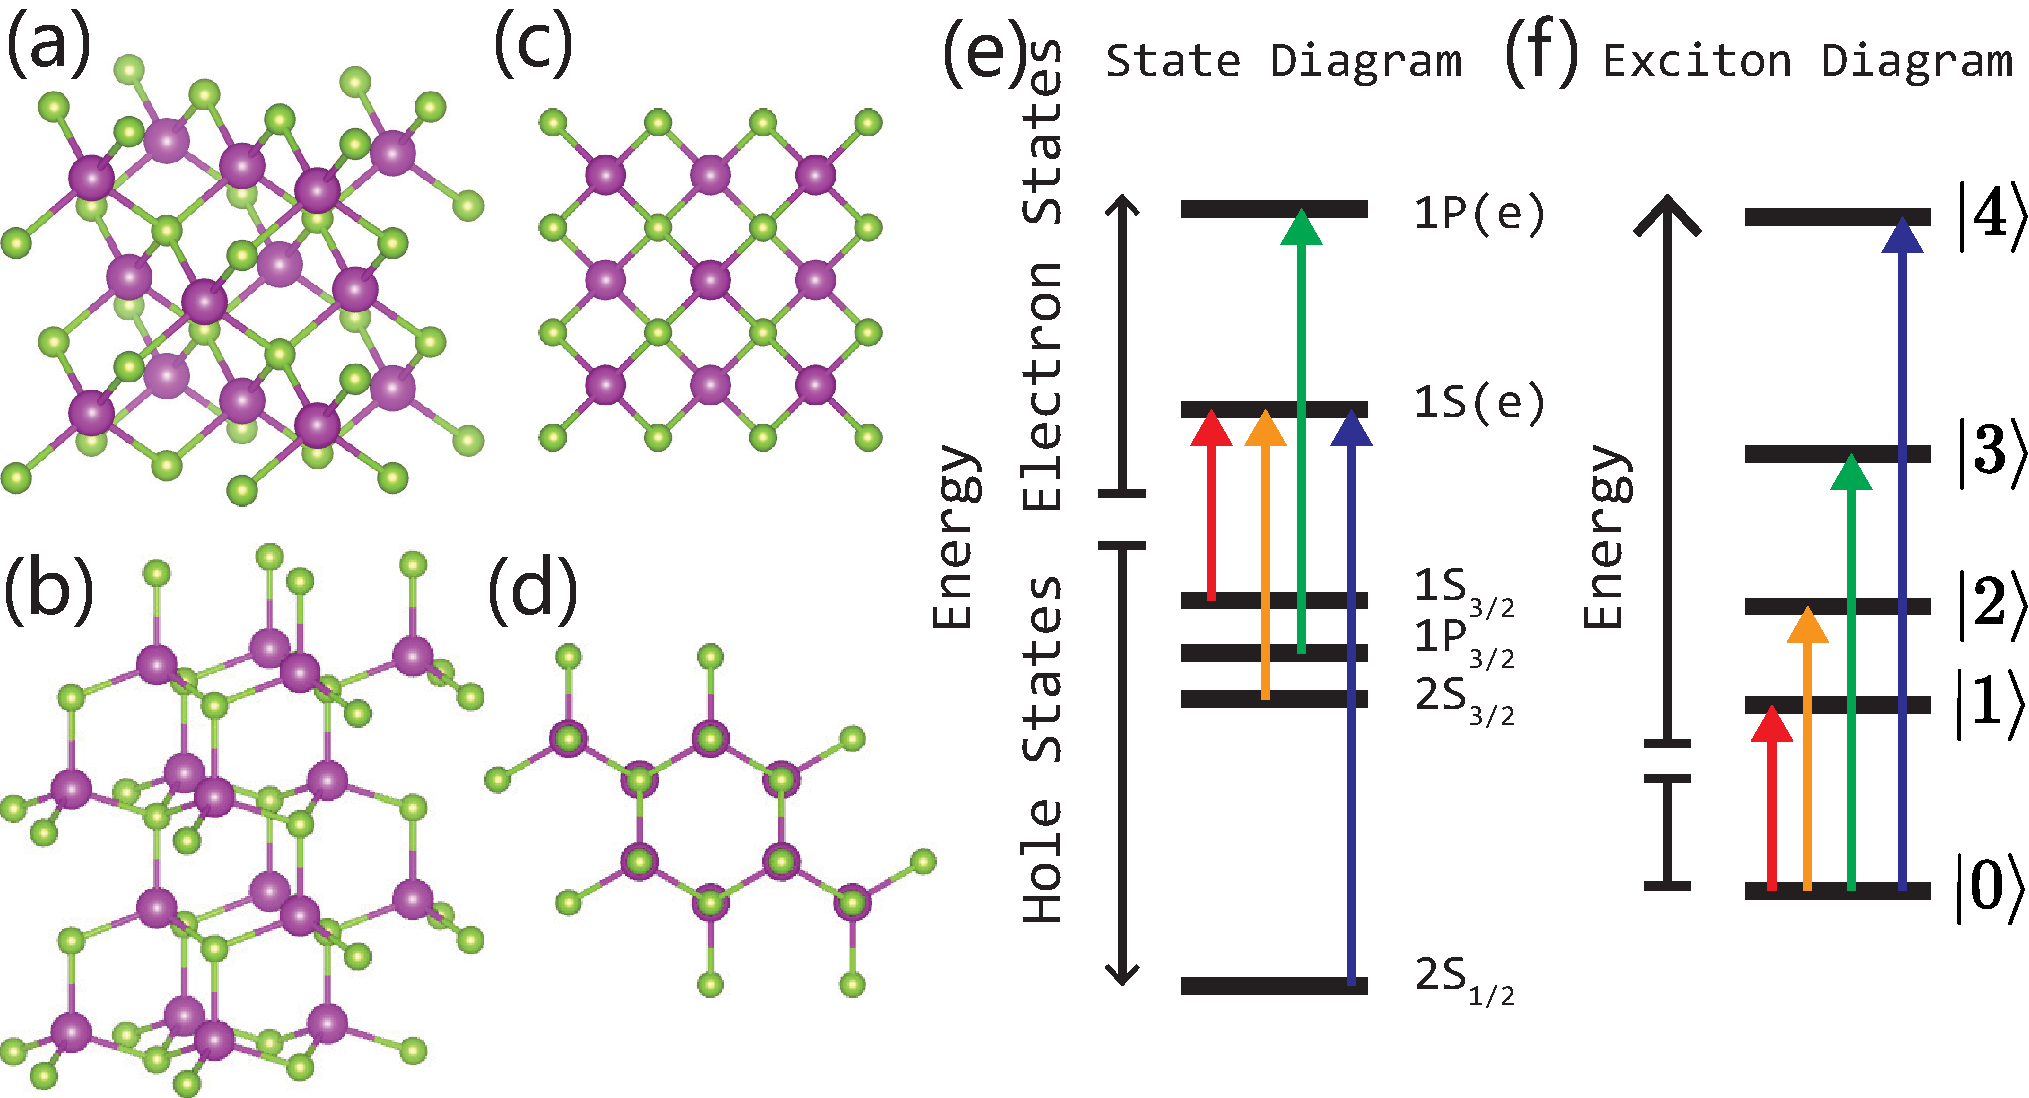
\includegraphics[width=.8\columnwidth]{CdSe Quantum Dot.pdf}
    \caption{(a)(b) 闪锌矿型和纤锌矿型 \ce{CdSe} 晶体结构;(c)(d) 闪锌矿型和纤锌矿型 \ce{CdSe} 晶体结构 $c$ 方向视图;(e) \ce{CdSe} 量子点的电子态和空穴态能级(改自 \cite{caram2014persistent});(f) \ce{CdSe} 量子点的激子能级(改自 \cite{caram2014persistent})。}
    \label{CdSe Quantum Dot}
\end{figure}

\chapter{实验结果与分析}
\section{实验装置}
本实验采用如图 \eqref{2D Spectrum System} 所示的装置,我们利用飞秒激光器(图 \ref{2D Spectrum System} \textcircled{\footnotesize{1}})作为激光源,产生重复频率为 $100$ kHz,波长为 $1030$ nm 的激光脉冲,输出总功率为 $40.000$ W,故每个激光脉冲携带有 $400$ $\mu$J 的能量,在时域上的宽度约 $?$ fs。每个激光脉冲由半透半反镜分为两束,一束经过光参量放大器(Optical Parametric Amplifier,简称 OPA,图 \ref{2D Spectrum System} \textcircled{\footnotesize{4}})转换为 $1280$ nm 波长后,通过厚度为 $1$ mm 的硼酸钡(Barium borate,化学式 \ce{Ba(BO2)2},简称 BBO,图 \ref{2D Spectrum System} \textcircled{\footnotesize{5}})晶体,利用 BBO 晶体的二次谐波产生(Second Harmonic Generation,简称 SHG)效应转换为 $640$ nm 波长,将其输入脉冲整形器(Pulse Shaper,图 \ref{2D Spectrum System} I),从而使单个脉冲重整为时间间隔可以调节的两个相邻脉冲,作为泵浦光(Pump Beam)照射样品(图 \ref{2D Spectrum System} \textcircled{\footnotesize{11}});另一路激光脉冲经过置于水平位移台(图 \textcircled{\footnotesize{11}})上的一对反射镜的反射,得到相对于泵浦脉冲的时延,再经一钇铝石榴石(Yttrium Aluminium Garnet,化学式 \ce{Y3Al5O12},简称 YAG)晶体通过非线性效应产生主要能量集中于 $540$ nm 至 $700$ nm 波段范围内的白光,作为探测光(Probe Beam)输入样品。探测光与泵浦光的光路交汇于样品的同一点,但探测光相对于泵浦光存在时延。在探测光传播方向上的单色仪(Monochrometer,图 \ref{2D Spectrum System} 左侧圆角矩形)将信号光在水平面上按照波长展开,用高速线扫描相机(图 \ref{2D Spectrum System} \textcircled{\footnotesize{11}})对各波长的信号进行采样。

\begin{figure}[h!]
    \centering
    \includegraphics[width=1\columnwidth]{2D Spectrum System.pdf}
    \caption{二维光谱系统. \textcircled{\footnotesize{1}} --- 激光源(Light Conversion Inc, CARBIDE - CB3),\textcircled{\footnotesize{2}} --- 平面反射镜,\textcircled{\footnotesize{3}} --- 半透半反镜,\textcircled{\footnotesize{4}} --- 光参量放大器(Light Conversion, ORPHEUS-TWINS),\textcircled{\footnotesize{5}} --- BBO 晶体,\textcircled{\footnotesize{6}} --- 水平位移台(Thorlabs, LTS300),\textcircled{\footnotesize{7}} --- 反射光栅,\textcircled{\footnotesize{8}} --- 离轴抛物柱面反射镜,\textcircled{\footnotesize{9}} --- 声光调制器,\textcircled{\footnotesize{10}} --- 非线性晶体,\textcircled{\footnotesize{11}} --- 样品,\textcircled{\footnotesize{12}} --- 线扫描相机(Teledyne e2v 公司, OCTOPLUS BA2),I --- 脉冲整形器(PhaseTech 公司, QuickShape Visible),II --- 光栅光谱仪(其中单色仪为北京卓立汉光仪器有限公司的 Omni-λ200i 系列)。}
    \label{2D Spectrum System}
\end{figure}

在脉冲整形器中,反射光栅将每个脉冲中不同波长的成分以不同角度反射,再由焦点位于反射光栅处的离轴抛物柱面反射镜反射而转换为平行光,从而实现对脉冲中不同波长的成分在空间上的分离。脉冲整形器的高速任意波发生器(Arbitrary Wave Generator,简称 AWG)将脉冲整形所需的掩模函数转换为含时射频信号,这一信号经过放大后驱动声光调制器(Acousto-optic Modulator,简称 AOM)中的压电换能器(Piezoelctric Transducer)以在 AOM 的 \ce{TiO2} 晶体中产生声波(密度疏密的空间分布),从而引起其折射率的空间分布,激光脉冲穿过这一特殊的“光栅”时就等效于对激光脉冲在频域进行调制。完成调制的激光脉冲再经过另一组对称的离轴抛物柱面反射镜和反射光栅的逆操作,即可在空间上重新合并为一束。在适合的信号激励下,可以使得最终输出时每个脉冲在时域上一分为二,并且带有给定的相位。通过调节 AOM 射频功率还可以控制泵浦光的强度。

我们通过改变 AOM 的折射率分布可以调节产生的每一对泵浦脉冲中两个脉冲间的时延 $\tau$,关于 $\tau$ 作傅里叶变换,得到的频率即为所谓二维光谱的其中一维。

每对泵浦脉冲之间的时延在数飞秒到数千飞秒的量级范围内进行扫描,此即产生的信号光相对于探测光的时延量级,而线扫描相机的采样周期和曝光时间均不低于纳秒量级,因此实验中线扫描相机的采样结果中同时包含了探测光和信号光的贡献。由于信号光的功率远小于探测光的功率,为了提取出信号光的有效信息并且提高信噪比,对于给定的 $\tau$,我们需要利用 AOM 对相邻两对泵浦脉冲依次交替施加 $0$ 相位和 $\pi$ 相位,从而使得相邻两次的信号光具有相反的振幅,将相邻两次线扫描相机的采样结果相减,即可抵消探测光的信号背底和其他噪声对采样结果的贡献,而仅保留信号光的有效信息。实际实验中,由于线扫描相机在对奇数行和偶数行采样时分别使用两组不同的像素点,为了避免使用不同的像素点而引入的误差,我们以 $4$ 对泵浦脉冲为一组,分别施加 $0$, $0$, $\pi$, $\pi$ 的相位,并且只取采样得到的奇数或偶数行的信号进行分析。

探测光的频率则构成了二维光谱的另一维。由单色仪和线扫描相机组装而成了光栅光谱仪,当探测光和信号光一同进入单色仪后,经一平面反射镜和离轴抛物柱面反射镜准直,被一反射光栅分光,将不同波长的成分在空间上分开,再经另一组离轴抛物柱面反射镜和平面反射镜汇聚于线扫描相机,经过换算可以将线扫描相机的像素点与光波长对应起来,从而得到光谱。

此外,通过调节水平位移台的前后移动,还可以改变探测光相对于泵浦光的时延 $T$,从而能够研究激发态的弛豫过程的快慢。

\section{待测样品}
本实验的样品采用自制的悬浮于正己烷(Hexane, 结构式 \ce{CH3CH2CH2CH2CH3})中的闪锌矿结构 \ce{CdSe} 量子点胶体,在此基础上通过用 \ce{Mn} 取代部分 \ce{Cd} 的方式制备了作为对照的 \ce{Cd_{1-x}Mn_xSe} (利用电感耦合等离子体发射光谱得到 $x=0.118$)量子点胶体。利用紫外可见吸收光谱仪分别测得 $10$ mm 厚的两种两种量子点胶体的吸光度与入射光子能量(波长)的关系如图 \ref{Absorption spectrum} 所示,其中两种样品的最低能量的信号峰,分别对应其从最高电子态至最低空穴态的跃迁,即 1S$_{3/2}\rightarrow$1S 跃迁,故两种样品的带隙分别为 $1.96$ eV 和 $2.41$ eV,对应激发波长分别为 $634$ nm 和 $516$ nm。

\begin{figure}[h]
    \centering
    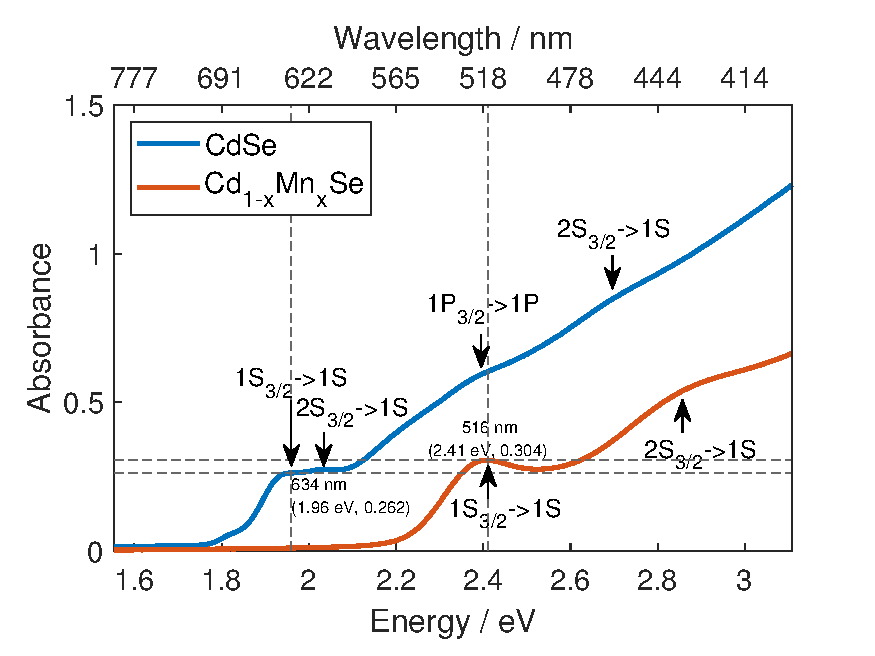
\includegraphics[width=.8\columnwidth]{Quantum-Dot-CdSe-and-Cd1-xMnxSe-Absorption-Spectrum.pdf}
    \caption{待测样品 \ce{CdSe} 量子点胶体和 \ce{Cd_{1-x}Mn_xSe} 量子点胶体的吸收谱。用辅助线标明的两个峰分别对应两种样品的 1S$_{3/2}\rightarrow$1S 跃迁。两个坐标仅分别为两个峰的极大值位置,而非通过拟合得到。}
    \label{Absorption spectrum}
\end{figure}

根据经验公式\cite{jasieniak2009re}
\begin{align}
    \notag D(\text{nm})=&59.60816-0.54736[\lambda(\text{nm})]+1.8873\times 10^{-3}[\lambda(\text{nm})]^2-2.85743\times 10^{-6}[\lambda(\text{nm})]^3\\
    &+1.62974\times 10^{-9}[\lambda(\text{nm})]^4,
\end{align}
得到量子点的直径为 $6.32$ nm。我们还尝试着使用布鲁斯公式估算了量子点的直径。对于闪锌矿型的体块 \ce{CdSe},带隙为 $1.74$ eV\cite{ninomiya1995optical,janowitz1994dielectric},电子和(重)空穴的有效质量分别为 $m_e^*=0.12 m_e$ 和 $m_h^*=0.9 m_e$($100$ 方向;其中 $m_e$ 为电子质量)\cite{kim1994optical},在波长为 $627.2$ nm (对应光子能量为 $1.982$ eV)的光下的相对介电常数 $\epsilon_r=8.0251$\cite{reshak2006theoretical},我们利用布鲁斯公式(式 \eqref{Brus Equ})计算得到 \ce{CdSe} 量子点的直径为 $6.70$ nm,与上面经验公式的计算结果相近。

在利用二维光谱系统对样品进行测量时,我们将 \ce{CdSe} 量子点胶体装于厚度为 $1.00$ mm 的石英比色皿(图 \ref{2D Spectrum System} \textcircled{\footnotesize{11}})中。

\section{泵浦功率的确定}
由于以上的理论限定于单激子激发的情形(Single-exciton Regime),但是当泵浦光强度很大时,可能发生一个量子点吸收超过一个光子,产生多激子激发的情形(Multi-exciton Regime),使问题复杂化。为了抑制多光子激发而保证单光子激发主导,我们需要泵浦光的强度低于某一阈值,而为了得到尽可能高的信噪比,我们又需要泵浦光的强度尽可能强。为此,我们需要确定一个最适宜的泵浦功率。

我们首先估算了单个量子点在每个脉冲中吸收的光子数。根据经验公式\cite{jasieniak2009re}
\begin{align}
    \varepsilon_{\text{1S}_{3/2}\text{(h)}\rightarrow\text{1S(e)}}(\text{mol}^{-1}\text{cm}^{-1})=155507+6.67054\times 10^{13}\exp\left(-\frac{E_{\text{1S}_{3/2}\rightarrow\text{1S(e)}}}{0.10551}\right),
\end{align}
计算得到 \ce{CdSe} 量子点胶体的 1S$_{3/2}\rightarrow$1S(e) 跃迁贡献的摩尔消光系数为 $7.22\times 10^5\text{mol}^{-1}$。摩尔消光系数和散射截面存在关系\cite{jasieniak2009re}
\begin{align}
    \varepsilon=\frac{N_A\times\sigma}{1000\times\ln(10)}
\end{align}
其中 $N_A$ 为阿伏伽德罗常数,故转换得到单颗 \ce{CdSe} 量子点的散射截面为 $\sigma=2.76\times 10^{-15}$ cm$^2$。

在 AOM 射频功率为 $20\%$ 的情况下,我们用功率计测量了通过直径为 $50$ $\mu$m 的针孔光阑的泵浦光的功率约为 $50$ $\mu$W,故每个泵浦脉冲的单位截面上的能量密度为 $1.27$ J/cm$^2$,单位截面上通过的光子数为 $4.10\times 10^{13}$ cm$^{-2}$,故平均每颗量子点吸收 $N=0.113$ 个光子。若将量子点吸收光子的过程建模为泊松过程,单颗量子点吸收光子数满足泊松分布,即单颗量子点吸收 $n$ 个光子的概率为
\begin{align}
    P(n)=\frac{N^n}{n!}exp{-N}.
\end{align}
由上式得到单个量子点在单个泵浦脉冲激发时吸收单个光子的概率为 $10.1\%$,而吸收两个光子的概率为 $0.6\%$,单光子吸收的概率远远高于双光子吸收的概率,因此当前泵浦光的强度应当可以保证单激子激发情形。

为了确保泵浦光与量子点胶体的相互作用是以单激子激发情形主导的,我们还测量了瞬态吸收谱。设定 AOM 射频强度为 $20\%$,设定 AOM 为 chop 模式,相邻两次探测中一次有泵浦光激发,一次无泵浦光,我们通过移动水平位移台来扫描探测光脉冲相对于泵浦脉冲的时延,得到如图 ? 所示的瞬态吸收谱,由图所示,当探测光脉冲相对于泵浦脉冲为负时延,即探测光脉冲先于泵浦脉冲到达样品时,探测光的透射强度较强,而当探测光脉冲相对于泵浦脉冲为正时延,即探测光脉冲晚于泵浦脉冲到达样品时,探测光的透射强度较弱,在零时延位置附近,探测光透射强度有一突变,由此我们确定,位移台位置为 $248.7$ mm 对应着探测光脉冲与泵浦脉冲零时延。

将位移台位置调至 $248.6$ mm,此时探测光脉冲相对于泵浦光脉冲的时延为 $0.67$ ps,通过调节 AOM 射频信号功率来改变泵浦脉冲的强度,得到脉冲光的透射率随 AOM 射频信号的变化关系,如图 ? 所示。

\chapter{结论}

\chapter{附录}
\section{刘维尔 - 冯诺依曼方程与双边费曼图}
\subsection{刘维尔 - 冯诺依曼方程的证明}
刘维尔 - 冯诺依曼方程是用于描述系统的密度矩阵随时间的演化的偏微分方程,可以由用于描述系统的量子态随时间演化的薛定谔方程推导得到。假设某系统在 $t$ 时刻的密度矩阵为
\begin{align}
    \hat{\rho}(t)=\sum_nP_n\lvert\psi_n(t)\rangle\langle\psi_n(t)\rvert,
\end{align}
其中某一纯态 $\lvert\psi_n(t)\rangle$ 随时间的演化遵循薛定谔方程,
\begin{align}
    \label{Shrodinger-Equ}
    \frac{\partial}{\partial t}\lvert\psi_n(t)\rangle=-\frac{i}{\hbar}\hat{H}\lvert\psi_n(t)\rangle,
\end{align}
其中 $\hat{H}(t)$ 为系统的哈密顿量,
则系统的密度矩阵随时间的演化遵循
\begin{align}
    \notag\frac{\partial}{\partial t}\hat{\rho}(t)=&\frac{\partial}{\partial t}\sum_nP_n\lvert\psi_n(t)\rangle\langle\psi_n(t)\rvert\\
    =&\sum_nP_n\left[\left(\frac{\partial}{\partial t}\lvert\psi_n(t)\rangle\right)\langle\psi_n(t)\rvert+\lvert\psi_n(t)\rangle\left(\frac{\partial}{\partial t}\lvert\psi_n(t)\rangle\right)^{\dagger}\right].
\end{align}
根据薛定谔方程(式 \eqref{Shrodinger-Equ}),用 $-\frac{i}{\hbar}\hat{H}$ 代替上式中的 $\frac{\partial}{\partial t}$,有
\begin{align}
    \notag\frac{\partial}{\partial t}\hat{\rho}(t)=&\sum_nP_n\left[-\frac{i}{\hbar}\hat{H}\lvert\psi_n(t)\rangle\langle\psi_n(t)\rvert+\lvert\psi_n(t)\rangle\left(-\frac{i}{\hbar}\hat{H}\lvert\psi_n(t)\rangle\right)^{\dagger}\right]\\
    \notag=&\sum_nP_n\left[-\frac{i}{\hbar}\hat{H}\lvert\psi_n(t)\rangle\langle\psi_n(t)\rvert+\frac{i}{\hbar}\lvert\psi_n(t)\rangle\langle\psi_n(t)\rvert\hat{H}\right]\\
    \notag=&-\frac{i}{\hbar}\left[\hat{H}\sum_nP_n\lvert\psi_i(t)\rangle\langle\psi_i(t)\rvert-\sum_nP_n\lvert\psi_n(t)\rangle\langle\psi_n(t)\rvert\hat{H}\right]\\
    =&-\frac{i}{\hbar}\left[\hat{H}\hat{\rho}(t)-\hat{\rho}(t)\hat{H}\right],
\end{align}
\begin{gather}
    \label{von Neumann Equ}
    \Longrightarrow i\hbar\frac{\partial}{\partial t}\hat{\rho}=[\hat{H},\hat{\rho}(t)].
\end{gather}
此即\textbf{刘维尔 - 冯诺依曼方程},其中 $[\cdots]$ 代表对易子,即 $[\hat{H},\hat{\rho}]=\hat{H}\hat{\rho}-\hat{\rho}\hat{H}$.

\subsection{刘维尔 - 冯诺依曼方程的求解}
上一小节中所列的为冯诺依曼方程在薛定谔绘景(Schrödinger Picture)中的形式。当系统的哈密顿量与时间有关,即系统的总哈密顿量可以表示为不含时的无微扰哈密顿量 $H_0$ 与含时的微扰哈密顿量 $\hat{H}_I(t)$ 之和,
\begin{align}
    \hat{H}(t)=\hat{H}_0+\hat{H}_I(t),
\end{align}
上述形式的冯诺依曼方程并不容易求解。为了便于求解冯诺依曼方程,我们首先需要暂时将其由薛定谔绘景转入相互作用绘景(Interaction Picture,又称狄拉克绘景,Dirac Picture),利用微扰理论求解得到相互作用绘景中的密度矩阵后,再将其转化回薛定谔绘景中。
在相互作用绘景中,任一可观测物理量 $O$ 的算符表示为
\begin{align}
    \hat{O}'(t)=\hat{U}_0(-t)\hat{O}(t)\hat{U}_0(t),
\end{align}
其中 $\hat{O}(t)$ 为可观测物理量 $O$ 的算符在薛定谔绘景中的形式,不含时无微扰哈密顿量对应的时间演化算符 $\hat{U}_0(t)=\exp\left[-\frac{i}{\hbar}\int_0^t\hat{H}_0\,\mathrm{d}\tau\right]$。
在相互作用绘景中,系统密度矩阵也可以用相似的方式表示为
\begin{align}
    \hat{\rho}'(t)=\hat{U}_0(-t)\hat{\rho}(t)\hat{U}_0(t).
\end{align}
其关于时间的演化遵循
\begin{align}
    \frac{\partial}{\partial t}\hat{\rho}'(t)=\left[\frac{\partial}{\partial t}\hat{U}_0(-t)\right]\hat{\rho}(t)\hat{U}_0(t)+\hat{U}_0(-t)\left[\frac{\partial}{\partial t}\hat{\rho}(t)\right]\hat{U}_0(t)+\hat{U}_0(-t)\hat{\rho}(t)\left[\frac{\partial}{\partial t}\hat{U}_0(t)\right],
\end{align}
其中
\begin{align}
    \notag\frac{\partial}{\partial t}\hat{U}_0(t)=&\frac{\partial}{\partial t}\exp\left[-\frac{i}{\hbar}\hat{H}_0t\right]=\frac{\partial}{\partial t}\sum_{n=0}^{\infty}\frac{1}{n!}\left[-\frac{i}{\hbar}\hat{H}_0t\right]^n=\sum_{n=1}^{\infty}\frac{1}{(n-1)!}\left[-\frac{i}{\hbar}\hat{H}_0\right]^nt^{n-1}\\
    =&-\frac{i}{\hbar}\hat{H}_0\sum_{n=0}\frac{1}{n!}\left[-\frac{i}{\hbar}\hat{H}_0t\right]^n=-\frac{i}{\hbar}\hat{H}_0\exp\left[-\frac{i}{\hbar}\hat{H}_0t\right]=-\frac{i}{\hbar}\hat{H}_0\hat{U}_0(t),
\end{align}
而
\begin{align}
    \frac{\partial}{\partial t}\hat{U}_0(-t)=-\frac{\partial}{\partial(-t)}\hat{U}_0(-t)=\frac{i}{\hbar}\hat{H}_0\hat{U}_0(-t),
\end{align}
以及根据刘维尔方程(式 \eqref{von Neumann Equ}),故有
\begin{align}
    \label{Density matrix evolution in interaction pic}
    \frac{\partial}{\partial t}\hat{\rho}'(t)=\frac{i}{\hbar}\hat{H}_0\hat{U}_0(-t)\hat{\rho}(t)\hat{U}_0(t)-\frac{i}{\hbar}\hat{U}_0(t)[\hat{H}_0(t)+\hat{H}_I(t),\hat{\rho}(t)]\hat{U}_0(t)-\frac{i}{\hbar}\hat{U}_0(-t)\hat{\rho}(t)\hat{H}_0\hat{U}_0(t).
\end{align}
由于 $\hat{U}_0(t)$ 可以展开为关于 $\hat{H}_0$ 的多项式,故 $\hat{U}_0(t)$ 与 $\hat{H}_0$ 对易,
\begin{align}
    \notag[\hat{U}_0(t),\hat{H}_0]=&\hat{U}_0\hat{H}_0-\hat{H}_0\hat{U}_0(t)=\exp\left[-\frac{i}{\hbar}\hat{H}_0t\right]\hat{H}_0-\hat{H}_0\exp\left[-\frac{i}{\hbar}\hat{H}_0t\right]\\
    =&\sum_{n=0}^{\infty}\frac{1}{n!}\left(-\frac{i}{\hbar}\hat{H}_0t\right)^n\hat{H}_0-\hat{H}_0\sum_{n=0}^{\infty}\frac{1}{n!}\left(-\frac{i}{\hbar}H_0t\right)^n=0.
\end{align}
因此式 \eqref{Density matrix evolution in interaction pic} 可以进一步化为
\begin{align}
    \notag\frac{\partial}{\partial t}\hat{\rho}'(t)=&\frac{i}{\hbar}\hat{H}_0\hat{U}_0(-t)\hat{\rho}(t)\hat{U}_0(t)-\frac{i}{\hbar}\hat{H}_0\hat{U}_0(-t)\hat{\rho}(t)\hat{U}_0(t)+\frac{i}{\hbar}\hat{U}_0(-t)\hat{\rho}(t)\hat{U}_0(t)\hat{H}_0\\
    \notag&-\frac{i}{\hbar}\hat{U}_0(-t)[\hat{H}_I(t),\hat{\rho}(t)]\hat{U}_0(t)-\frac{i}{\hbar}\hat{U}_0(-t)\hat{\rho}(t)\hat{U}_0(t)\hat{H}_0\\
    =&-\frac{i}{\hbar}\hat{U}_0(-t)[\hat{H}_I(t),\hat{\rho}(t)]\hat{U}_0(t).
\end{align}
向上式中插入单位算符 $\hat{1}=\hat{U}_0(t)\hat{U}_0(-t)$,可以将式中的微扰哈密顿量 $\hat{H}_I$ 和密度矩阵 $\hat{\rho}$ 均转化为相互作用表象中的形式,
\begin{align}
    \notag\frac{\partial}{\partial t}\hat{\rho}'(t)=&-\frac{i}{\hbar}\hat{U}_0(-t)\hat{H}_I(t)\hat{1}\hat{\rho}(t)\hat{U}_0(t)+\frac{i}{\hbar}\hat{U}_0(-t)\hat{\rho}(t)\hat{1}\hat{H}_I(t)\hat{U}_0(t)\\
    \notag=&-\frac{i}{\hbar}\hat{U}_0(-t)\hat{H}_I(t)\hat{U}_0(t)\hat{U}_0(-t)\hat{\rho}(t)\hat{U}_0(t)+\frac{i}{\hbar}\hat{U}_0(-t)\hat{\rho}_0(t)\hat{U}_0(t)\hat{U}_0(-t)\hat{H}_I(t)\hat{U}_0(t)\\
    =&-\frac{i}{\hbar}\hat{H}_I'(t)\hat{\rho}'(t)-\frac{i}{\hbar}\hat{\rho}'(t)\hat{H}_I'(t),
\end{align}
其中 $\hat{H}_I'(t)=\hat{U}_0(-t)\hat{H}_I(t)\hat{U}_0(t)$ 为相互作用绘景中的含时微扰哈密顿量。由此,我们得到相互作用绘景中的冯诺依曼方程为
\begin{align}
    \frac{\partial}{\partial t}\hat{\rho}'(t)=-\frac{i}{\hbar}[\hat{H}_I'(t),\hat{\rho}'(t)].
\end{align}
类似微扰力理论的处理方法,我们引入一个无量纲的系数 $\lambda$,将系统的总哈密顿量改写为
\begin{align}
    \hat{H}(t)=\hat{H}_0+\lambda\hat{H}_I(t).
\end{align}
我们将密度矩阵展开为关于 $\lambda$ 的级数,
\begin{align}
    \hat{\rho}'(t)=\hat{\rho}^{(0)}(t)+\lambda\hat{\rho}^{(1)}(t)+\lambda^2\hat{\rho}^{(2)}(t)+\cdots,
\end{align}
其中 $\hat{\rho}^{(n)}(t)$ 为密度矩阵对微扰的第 $n$ 阶修正项。
将上式代入相互作用绘景中的冯诺依曼方程,
\begin{align}
    \frac{\partial}{\partial t}[\hat{\rho}'^{(0)}(t)+\lambda\hat{\rho}'^{(1)}(t)+\lambda^2\hat{\rho}'^{(2)}(t)+\cdots]=-\frac{i}{\hbar}[\lambda\hat{H}_I'(t),\hat{\rho}'^{(0)}(t)+\lambda\hat{\rho}'^{(1)}(t)+\lambda^2\hat{\rho}'^{(2)}(t)+\cdots],
\end{align}
并对两边同阶级数的系数取等得
\begin{align}
    \frac{\partial}{\partial t}\hat{\rho}'^{(0)}(t)=&0,\\
    \frac{\partial}{\partial t}\hat{\rho}'^{(1)}(t)=&-\frac{i}{\hbar}[\hat{H}_I',\hat{\rho}'^{(0)}(t)],\\
    \notag\cdots&\\
    \frac{\partial}{\partial t}\hat{\rho}'^{(0)}(t)=&-\frac{i}{\hbar}[\hat{H}_I',\hat{\rho}'^{(n-1)}(t)],\\
    \notag\cdots&
\end{align}
对上面各式积分得由密度矩阵低阶修正项推算高阶修正项的递归式,
\begin{align}
    \hat{\rho}'^{(0)}(t)=&0,\\
    \hat{\rho}'^{(1)}(t)=&-\frac{i}{\hbar}\int_0^t[\hat{H}_I'(t),\hat{\rho}'^{(0)}(t)]\,\mathrm{d}\tau,\\
    \notag\cdots&\\
    \hat{\rho}'^{(n)}(t)=&-\frac{i}{\hbar}\int_0^t[\hat{H}(\tau),\hat{\rho}'^{(n-1)}(\tau)]\,\mathrm{d}\tau,\\
    \notag\cdots&
\end{align}
综合以上各递归式,有
\begin{align}
    \hat{\rho}'^{(0)}(t)=&\hat{\rho}'^{(0)}(t=0),\\
    \notag\hat{\rho}'^{(n)}(t)=&\left(-\frac{i}{\hbar}\right)^n\int_0^t\mathrm{d}\tau_1\int_0^{\tau_1}\mathrm{d}\tau_2\cdots\int_0^{\tau_{n-1}}\mathrm{d}\tau_{n-1}\,\left[\hat{H}_I'(\tau_1),\left[\hat{H}_I'(\tau_2),\cdots\left[\hat{H}_I'(\tau_n),\hat{\rho}'^{(0)}(\tau_n)\right]\cdots\right]\right]\\
    \notag=&\left(-\frac{i}{\hbar}\right)^n\int_0^t\mathrm{d}\tau_1\int_0^{\tau_1}\mathrm{d}\tau_2\cdots\int_0^{\tau_{n-1}}\mathrm{d}\tau_n\,\left[\hat{H}_I'(\tau_1),\left[\hat{H}_1'(\tau_2),\cdots\left[\hat{H}_I'(\tau_n),\hat{\rho}'^{(0)}(0)\right]\cdots\right]\right],\\
    &\forall n\geq 1.
\end{align}
将密度矩阵由相互作用绘景转化回薛定谔绘景中,得
\begin{align}
    \label{von Neumann Equ sol-1}
    \hat{\rho}^{(0)}(t)=&\hat{U}_0(t)\hat{\rho}^{(0)}(0)\hat{U}_0(-t),\\
    \label{von Neumann Equ sol-2}
    \notag\hat{\rho}^{(n)}(t)=&\hat{U}_0(t)\hat{\rho}'^{(n)}(t)\hat{U}_0(-t),\\
    \notag=&\left(-\frac{i}{\hbar}\right)^n\hat{U}_0(t)\int_0^t\mathrm{d}\tau_1\int_0^{\tau_1}\mathrm{d}\tau_2\cdots\int_0^{\tau_{n-1}}\mathrm{d}\tau_n\,\times\\
    &\left[\hat{H}_I'(\tau_1),\left[\hat{H}_I'(\tau_2),\cdots\left[\hat{H}_I'(\tau_n),\hat{\rho}^{(0)}(0)\right]\cdots\right]\right]\hat{U}_0(-t),\quad\forall n\geq 1.
\end{align}

\subsection{刘维尔 - 冯诺依曼方程的解与双边费曼图的对应关系}
冯诺依曼方程的解的高阶修正项(式 \eqref{von Neumann Equ sol-2})中含有嵌套的对易子,因此其项数随阶数呈现指数式的增长
更高阶数的修正项,对应着更高阶数的非线性效应。

\backmatter% initialize the environment
\intotoc{\bibname}% add link to contents table and bookmark
\bibliography{Biblio/ref}% bibliography

\chapter*{致谢}
谢天谢地!这篇论文到这里总算是要画上句号了,然而受了这么多人的帮助,那可得好好说一说。

Here, I should express my appreciation for Professor McGuire in the first place, who is responsible for guiding my senior thesis project. Your help to me does not only begin from this project, but dates back to the spring of 2020 when I take your Non-linear Optics course. It is one of the toughest course I have gone through in my undergraduate years, but also the most useful ones.

紧接着要感谢的必须是梁超逸师兄。在二维光谱的项目中师兄承担了仪器搭建、程序设计、设备维护等一系列困难而繁重的工作,可以说我在该项目上所花的时间精力不及师兄的零头。为了即时得到我们的数据,甚至占用了师兄的非工作时间,甚是抱歉。梁超逸师兄无论在物理原理还是实验技术上都有着超出同龄人的功底,在今后的研究生阶段,梁超逸师兄将是我努力学习的榜样。同时,课题组里的徐小凡、王凯、杜成江等各位师兄都对我的毕业论文给予了无私的帮助,在此一并表示感谢。

此外,当然要没有各位同学和朋友的陪伴和鼓励,那么完成这个课题的体验也将大打折扣。这里要感谢的是和我共同参与二维光谱项目的王晴宇同学以及时常和我聊天的高中同学黄鹏豪,你们缓解了我工作时间的沉闷与压力。

最后,感谢爸爸妈妈还有我自己。。。。

在将来的真正的科研生涯中,不求顺风顺水,但求能遇到向大家一样优秀而善良的人。

\end{document}